%%%%%%%%%%%%%%%%%%%%%%%%%%%%%%%%%%%%%%%%%%%%%%%%
\chapter{Produtos Notáveis}

Produtos notáveis são multiplicações algébricas que ocorrem com frequência. 

\section{Quadrado da soma}

\begin{equation}
(a+b)^2=a^2+2ab+b^2
\end{equation}

\subsection{Justificativa Geométrica}
\begin{figure}[h]
    \centering
    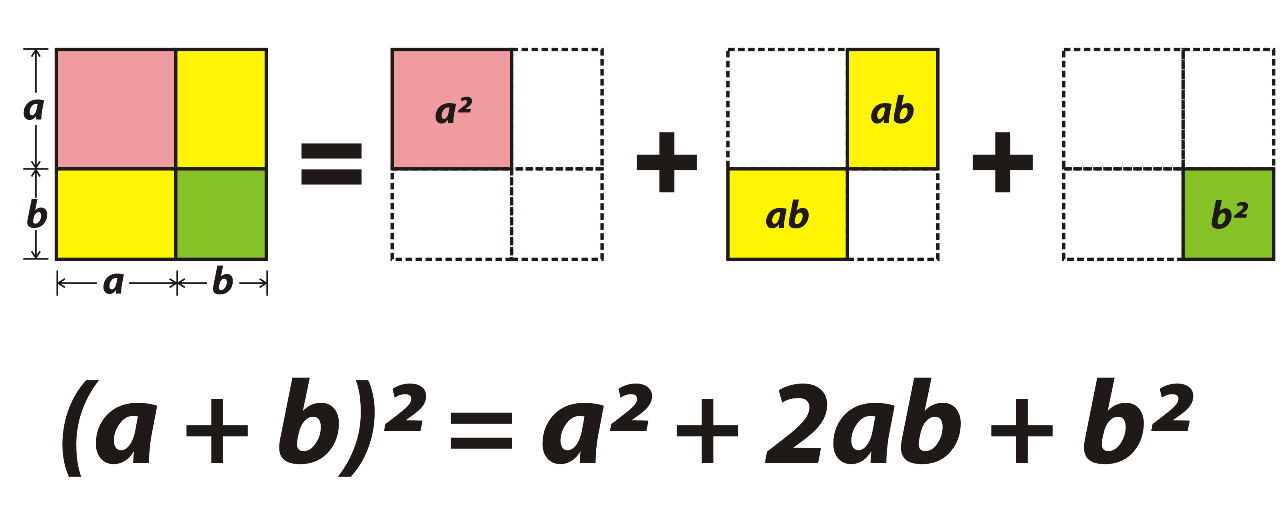
\includegraphics[scale=1]{./imagens/12.png}
    \caption{Quadrado da Soma}
    \label{fig:my_label}
\end{figure}

\section{Quadrado da Diferença}

\begin{equation}
(a-b)^2=a^2-2ab+b^2
\end{equation}

\section{Produto da soma pela diferença}

\begin{equation}
(a+b)(a-b)=a^2+b^2
\end{equation}

\subsection{Justificativa Geométrica}
\begin{figure}[h]
    \centering
    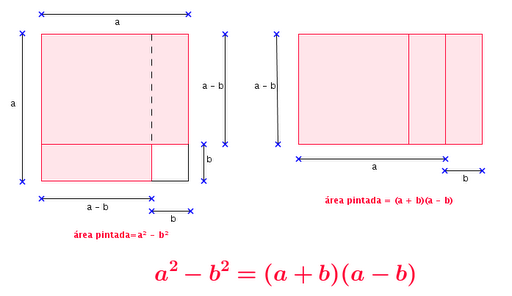
\includegraphics[scale=.6]{./imagens/29.png}
    \caption{Produto da soma pela diferença}
    \label{fig:my_label}
\end{figure}

\section{Cubo da soma}

\begin{equation}
(a+b)^3=a^3+3a^2+3ab^2+b^3
\end{equation}

\subsection{Justificativa Geométrica}

\begin{figure}[h]
    \centering
    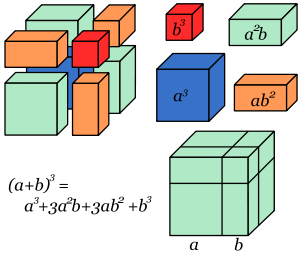
\includegraphics[scale=.5]{./imagens/13.png}
    \caption{Cubo da Soma}
    \label{fig:my_label}
\end{figure}

\section{Cubo da diferença}

\begin{equation}
(a-b)^3=a^3-3a^2+3ab^2-b^3
\end{equation}
